
\chapter{Dasar Teori}
\label{chap:Dasar Teori}
Pada bab ini diuraikan teori-teori yang berhubungan dengan pembangunan pohon kurikulum. Teori-teori tersebut adalah teori tentang pengertian Data Mata Kuliah Kurikulum, JSON, \textit{DOT language}, dan visualisasi pohon menggunakan \textit{viz.js}.

\section{Data Mata Kuliah Kurikulum}
\label{sec: Data Mata Kuliah Kurikulum}


\section{JSON}
\label{sec: JSON}

JSON \textit{(JavaScript Object Notation)} adalah format pertukaran data. \textit{JSON} merupakan format teks yang tidak bergantung pada bahasa pemprograman apapun.\footnote{"JSON", \url{https://www.json.org/json-id.html}} Kenapa \textit{JSON}? Karena ukuran datanya lebih kecil dibanding dengan \textit{XML}, sifatnya \textit{"self-describing"} dan mudah dimengerti. Formatnya berbasis teks dan terbaca manusia serta digunakan untuk mempresentasikan struktur data sederhana. Format teks dari JSON itu sendiri identik dengan kode untuk membuat objek \textit{JavaScript} memiliki kesamaan dengan \textit{Javascript}, hanya saja \textit{JSON} lebih mudah dimengerti. 

\subsection{Struktur JSON}
\label{sec: Struktur JSON}
JSON terbuat dari dua struktur:
\begin{enumerate}
\item Kumpulan pasangan nama/nilai. Pada beberapa bahasa, hal ini dinyatakan sebagai objek \textit{(object)}, rekaman \textit{(record)}, struktur \textit{(struct)}, kamus \textit{(dictionary)}, tabel hash\textit{(hash table)}, daftar berkunci \textit{(keyed list)}, atau \textit{associative array}.
\item Daftar nilai terurutkan \textit{(an ordered list of values)}. Pada kebanyakan bahasa, hal ini dinyatakan sebagai larik \textit{(array)}, vektor \textit{(vector)}, daftar \textit{(list)}, atau urutan \textit{(sequence)}. 
\end{enumerate}

\textit{JSON} menggunakan bentuk sebagai berikut:
\begin{enumerate}
\item \textbf{Objek} adalah sepasang nama/nilai yang tidak terurutkan. Objek dimulai dengan "{" dan "}". Setiap nama diikuti dengan ":: dan setiap pasangan nama/nilai dipisahkan oleh ",". Contohnya seperti pada Gambar \ref{fig: objek}.
\begin{figure}[H]
		\centering
		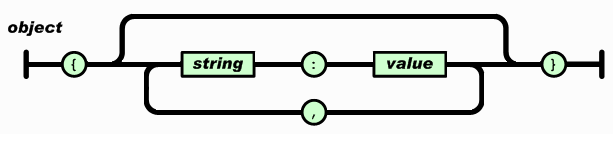
\includegraphics[scale = 0.5]{1.png}
		\caption{JSON berbentuk Objek}
		\label{fig: objek}
\end{figure}	

\item \textbf{Larik} adalah kumpulan nilai yang terurutkan. Larik dimulai dengan "[" dan diakhiri dengan "]". Setiap nilai dipisahkan oleh ",". Contohnya seperti pada Gambar \ref{fig: larik}.
\begin{figure}[H]
		\centering
		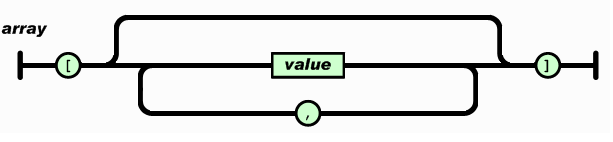
\includegraphics[scale = 0.5]{2.png}
		\caption{JSON berbentuk Larik}
		\label{fig: larik}
\end{figure}	

\item \textbf{Nilai}, dapat berupa sebuah \textit{string} dalam tanda kutip ganda, atau angka, atau true atau false atau null, atau sebuah objek atau sebuah larik. Struktur-struktur tersebut dapat disusun bertingkat. Contohnya seperti pada Gambar \ref{fig: nilai}.
\begin{figure}[H]
		\centering
		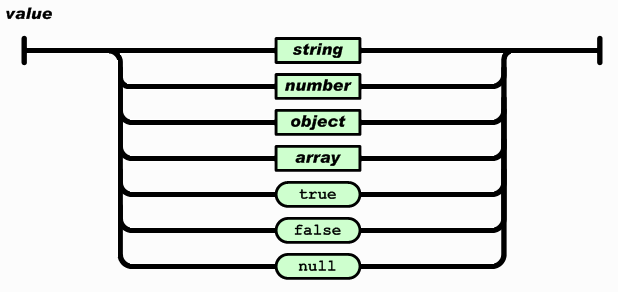
\includegraphics[scale = 0.5]{3.png}
		\caption{Nilai yang dapat dimasukan ke dalam JSON}
		\label{fig: nilai}
\end{figure}	


\end{enumerate}

\subsection{Contoh Sintaks}
\label{sec: Contoh Sintaks}
Contoh berikut menunjukkan representasi JSON untuk suatu objek yang mendeskripsikan seseorang.
\begin{lstlisting}
{ 
"namaDepan": "Budi", 
"namaBelakang": "Subudi", 
"alamat": { 
	"namaJalan": "Jl. Sudirman 15A", 
	"kota": "Jakarta Selatan", 
	"provinsi": "DKI Jakarta", 
	"kodePos": 11111 }, 
	"nomerTelepon": [ 
	"021 555-1234", 
	"021 555-4567" 
	] 
}
\end{lstlisting}

\section{DOT Language}
\label{sec: DOT Language}

\textit{DOT} adalah bahasa yang dapat digunakan untuk menampilkan grafik secara teks, sehingga dapat diproses melalui titik untuk membuat grafik sebagai representasi grafis dalam format yang berbeda seperti .ps, .pdf, dll.~\cite{north:03:DOT} DOT telah dikembangkan sebagai bagian dari proyek \textit{Graphviz}, yang merupakan kumpulan alat untuk visualisasi grafik. 

\subsection{Dasar Menggambar Graf}
\label{sec: Dasar Menggambar Graf}
Dot mengambil empat langkah utama dalam menggambar grafik. Langkah pertama menetapkan diskrit peringkat ke node dalam gambar atas ke bawah, menentukan peringkat di koordinat Y. Tepi yang membentang lebih banyak dari satu peringkat dipecah menjadi rantai simpul dan tepi unit. Langkah kedua \textit{node} dalam barisan untuk menghindari penyeberangan. Langkah ketiga menetapkan koordinat \textit{node} X untuk disimpan dibaris terpendek. Langkah terakhir rute tepi splines. Grafik menggunakan dot memiliki tiga jenis \textit{item}: grafik, simpul, dan tepi. Grafik sendiri memiliki dua bentuk yaitu grafik (tidak diarahkan) atau digraf (diarahkan). Karena dot membuat \textit{layout} grafik yang diarahkan maka contoh dalam kasus ini menggunakan digraf. 

Gambar \ref{fig: contoh} adalah contoh grafik dalam bahasa dot. Baris 1 memberi nama dan jenis grafik. Baris berikut membuat node, tepi, atau subgraf, dan atur atribut. Nama merupakan \textit{identifier} C, nomor, atau kutipan C. Sebuah simpul diciptakan pertama kali namanya muncul di \textit{file}. Tepian dibuat saat node berada bergabung dengan operator tepi ->. Pada contoh, baris 2 membuat tepi lalu mengurai dari \textit{parse} ke \textit{execute}. Untuk menjalankan dot pada file ini (dimisalkan graf1.dot) dapat mengetikan $ dot -Tps graf1.dot -o graf1.ps $ dan akan menghasilkan Gambar \ref{fig: contoh}. 
\begin{lstlisting}
1: digraph G {
2: main -> parse -> execute;
3: main -> init;
4: main -> cleanup;
5: execute -> make_string;
6: execute -> printf
7: init -> make_string;
8: main -> printf;
9: execute -> compare;
10: }
\end{lstlisting}

\begin{figure}[H]
		\centering
		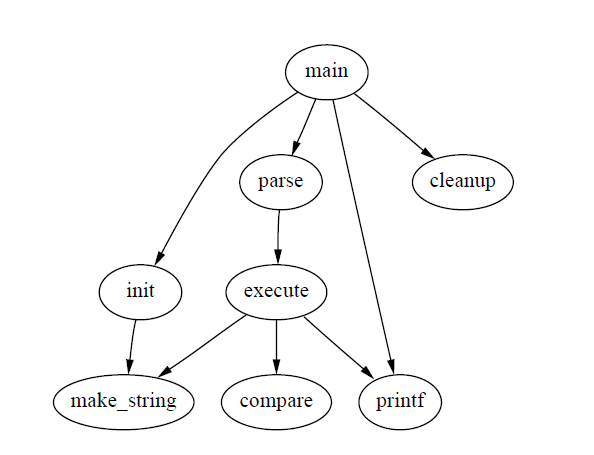
\includegraphics[scale = 0.5]{graph1.png}
		\caption{Contoh sederhana penggunaan graf}
		\label{fig: contoh}
\end{figure}	

Penjelasan sintaks di atas sebagai berikut:
\begin{enumerate}
\item \textbf{Digraph}, berfungsi untuk menunjukkan bahwa isi dari sintaks di atas akan berbentuk graf.
\item Pada sintaks terdapat kata-kata seperti \textit{main, parse, int,} dan lainnya. Kata-kata tersebut menunjukkan \textit{node} pada graf.
\item Setelah mengetahui \textit{node}, maka terdapat tanda "->" yang menunjukkan \textit{edge} dari setiap \textit{node}.
\end{enumerate}

\subsection{Subgraf dan Pengelompokan}
\label{sec: Subgraf dan Pengelompokan}
Subgraf memiliki tiga peran di \textit{Graphviz}. Pertama, subgraf dapat digunakan untuk mewakili struktur grafik, yang menunjukkan bahwa simpul dan tepi tertentu harus dikelompokkan bersama. Informasi pada subgraf ditentukan secara semantik tentang komponen grafik. Tepi dibuat dari setiap simpul di sebelah kiri ke setiap simpul di sebelah kanan. Contohnya sebagai berikut:
\begin{lstlisting}
A -> {B C} 

sama dengan
A -> B
A -> C
\end{lstlisting}

Pada saat menjalankan sintaks di atas akan menghasilkan Gambar \ref{fig: subgraf}.

\begin{figure}[H]
		\centering
		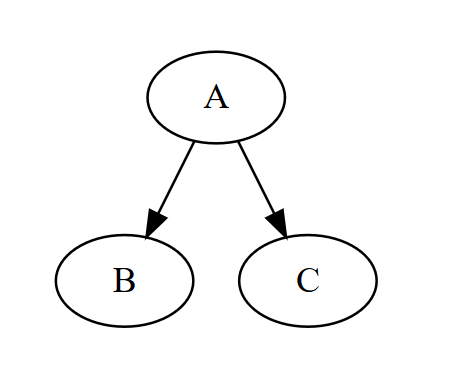
\includegraphics[scale = 0.3]{cA.png}
		\caption{Contoh sederhana subgraf}
		\label{fig: subgraf}
\end{figure}	


Kedua, subgraf dapat memberikan konteks untuk mengatur atribut. Sebagai contoh, sebuah subgraf dapat menentukan bahwa warna biru adalah warna \textit{default} untuk semua node yang didefinisikan di dalamnya. Dalam konteks gambar grafik, contohnya sebagai berikut

\begin{lstlisting}
subgraf {
peringkat = sama; A; B; C;
}
\end{lstlisting}

Subgraf ini menentukan bahwa simpul A, B dan C semuanya harus ditempatkan pada rangking yang sama jika ditarik menggunakan titik.

Ketiga untuk subgraf secara langsung melibatkan bagaimana grafik akan ditata oleh mesin. Jika nama subgraf dimulai dengan \textit{cluster}, \textit{Graphviz} mencatat subgraf sebagai subgraf \textit{cluster} khusus. Jika didukung, mesin akan melakukan tata letak sehingga simpul milik cluster digambar bersama, dengan keseluruhan gambar cluster yang ada di dalam persegi panjang yang melintang. Subgraf \textit{cluster} bukan bagian dari bahasa DOT, namun hanya konvensi sintaks yang dipatuhi oleh mesin.  


\subsection{Atribut Menggambar}
\label{sec: Atribut Menggambar}
Dalam membuat graf dibutuhkan beberapa atribut untuk menyempurnakan gambar. Atribut tersebut berisi 
\begin{enumerate}
\item Bentuk dan Label.\\
Pada bentuk dan label nantinya akan ditentukan \textit{node} akan berbentuk apa dan label pada node akan berisi apa. Secara \textit{default} bentuk dari node sendiri adalah elips. Tetapi ada bentuk lain yang diberikan untuk \textit{node} yaitu kotak, lingkaran, polygon, dll. 
\item Tampilan Graf\\
Simpul dan tepi memiliki atribut warna dan gaya. Penggunaan warna dalam membuat graf memiliki beberapa syarat. Pertama hindari menggunakan terlalu banyak warna cerah. Kedua, ketika node dipenuhi warna gelap label nampaknya lebih mudah dibaca dengan \textit{fontcolor} = putih dan \textit{fontname} = \textit{Helvetica}. Ketiga, menentukan ruang warna dengan mendefinisikan \textit{nodecolor}, \textit{edgecolor}, atau \textit{graphcolor} dalam file library. Misalnya, untuk menggunakan warna RGB, letakkan baris berikut di file lib.ps. / nodecolor {setrgbcolor} bind def. Gunakan opsi baris perintah -l untuk memuat file ini. $ dot -Tps -l lib.ps file.dot -o file.ps $
\item Ukuran Gambar dan Jarak\\
Seringkali gambar yang dibuat dengan ukuran dan pemisahan \textit{nodes default} terlalu besar untuk target atau untuk ruang yang diizinkan untuk gambar dalam dokumen. Ada beberapa cara untuk mencoba mengatasi masalah ini. Pertama, melihat bagaimana titik pada ukuran tata letak akhir. Tata letak awalnya dibuat secara internal dengan ukuran awal, dengan menggunakan pengaturan \textit{default}. Secara default, \textit{nodes} paling sedikit 0,75 inci dengan lebar 0,5; \textit{font} adalah 14, \textit{nodes} dipisahkan paling sedikit 0,25 dan diberi peringkat oleh 0,5 Tidak ada batasan ukuran atau aspek rasio gambar, jadi jika grafiknya besar, tata letaknya juga besar. Jika tidak menentukan ukuran atau rasio, maka ukuran awal akan dicetak. Cara termudah untuk mengontrol ukuran output gambar adalah dengan mengatur ukuran = x; y pada file grafik (atau pada baris perintah menggunakan -G). Ini menentukan kotak pembatas tata letak akhir. 

Tabel untuk atribut menggambar sebagai berikut:
\begin{enumerate}
\item \textit{Node Attributes}, Pada Tabel di bawah ini menunjukkan apa saja isi dari \textit{Node Attributes}
\begin{table}[H]
\begin{center}
\caption{\textit{Node Attributes}}
\begin{tabular}{|c|c|l|}
\hline
  Nama & Default & Value \\
\hline
  color & black & warna bentuk node \\
  fontcolor & black & warna huruf \\
  fontname & times-roman & jenis font \\
  fontsize & 14 & ukuran dari font \\
  height, width & .5,.75 & tinggi dan panjang dalam bentuk inchi \\
  label & node name & kalimat \\
  layer & overlay range & semua id \\
  shape & ellipse & ellipse, box, circle, doublecircle, plaintext, polygon \\
  shapefile & & external EPSF file if epsf shape \\
  style & & graphics options (bold, dotteed, filled)\\
\hline
\end{tabular}
\end{center}
\end{table}

\item \textit{Edge Attributes}, Pada Tabel di bawah ini menunjukkan apa saja isi dari \textit{Edge Attributes} \\

\begin{table}[H]
\begin{center}
\caption{\textit{Edge Attributes}}
\begin{tabular}{|c|c|l|}
\hline
  Nama & Default & Value \\
\hline
  color & black & warna garis \\
  decorate & & gambar yang menghubungkan label \\
  dir & forward & forward, back, both, or none \\
  fontcolor & black & warna forn \\
  fontname & times-roman & jenis font \\
  fontsize & 14 & ukuran fonr \\
  id & & optional value \\
  label & & label, if not empty \\
  layer & overlay range & all id \\
  minlen & 1 & minimum rank distance between head and tail \\
  style & & graphics options (bold, dotteed, filled) \\
  weight & 1 & integer reflecting inmportance of edge \\
\hline
\end{tabular}
\end{center}
\end{table}

\item \textit{Graph Attributes}, Pada Tabel di bawah ini menunjukkan apa saja isi dari \textit{Graph Attributes}

\begin{table}[H]
\begin{center}
\caption{\textit{Graph Attributes}}
\begin{tabular}{|c|c|l|}
\hline
  Nama & Default & Value \\
\hline
  center & & when true, centers drawing on page \\
  cluster rank & local & may be global or none \\
  color & black & node shape color \\
  fontcolor & black & type face color \\
  fontname & times-roman & PostScript font family \\
  fontsize & 14 & point size of label \\
  label & & any string \\
  layerseq & & id:id:id \\
  margin & .5,.5 & margin include in pages \\
  mclimit & 1.0 & if set to f adjusts mincross iterations by (f) \\
  nodesep & .25 & separation between nodes in inches \\
  ordering & & out (for ordered edges) \\
  page & & unit of pagination  \\
  rank & & same, min, max \\
  rankdir & TB & LR(left to right) or TB(top to bottom) \\
  ranksep & .75 & separation between ranks in inches \\
  ratio & & aprroximate aspect ratio desired \\
  size & & drawing bounding box in inches \\
\hline
\end{tabular}
\end{center}
\end{table}

\end{enumerate}
\end{enumerate}



\section{Visualisasi Graf dengan Viz.js}
\label{sec: Visualisasi Graf dengan Viz.js}

JSON sebagai salah satu format terbuka digunakan untuk membuat graf. Graf ini dihasilkan dengan menggunakan \textit{viz.js} yang merupakan mesin pembaca \textit{DOT}. \textit{DOT} sendiri dibuat dengan melihat struktur JSON. Agar graf dapat ditampilkan pada suatu \textit{web browser}, salah satu caranya adalah dengan menggunakan \textit{viz.js}. Visualisasi ini dapat dilakukan dengan menggunakan javascript dan HTML5 untuk membuat sebuah graf pada halaman \textit{web}. Hal pertama yang perlu dilakukan adalah dengan melakukan
\textit{install viz.js} di \url{https://github.com/mdaines/viz.js/releases}.\footnote{"viz", \url{https://github.com/mdaines/viz.js/releases}} Lalu data tersebut
diletakan pada \textit{file} yang akan digunakan. Berikut adalah contoh dalam menggunakan viz.js.
\begin{lstlisting}
1. <html>
2.    <body>
3.      <div id="graph"></div>
4.        <script src="assets/js/jquery.js"></script>
5.        <script src="assets/js/viz.js"></script>
6.        <script>
7.            $.get('kurikulum.dot', function (res) {
8.                var graph = Viz(res, { format: "svg", engine: "dot" });
9.                $("#graph").append(graph);
10.            })
11.        </script>
12.    </body>
13. </html>
\end{lstlisting}

Terdapat beberapa opsi parameter yang dapat digunakan untuk merubah tampilan dari graf
yang akan ditampilkan, yaitu:
\begin{itemize}
\item \textit{format} menetapkan \textit{format} keluaran, dan hasilnya salah satu dari "svg", "xdot", "plain", "ps", "json", atau "png-image-element". 
\item \textit{engine}, mengatur mesin \textit{Graphviz} untuk digunakan, salah satunya "circo", "dot", "fdp", "neato", "osage", or "twopi".
\end{itemize}


\section{Graf}
\label{sec: graf}